
%================2.1
% \section{Bài toán phân loại hai lớp}

Xét bài toán phân loại hai lớp $C_1$ và $C_2$. Mỗi đối tượng cần phân loại được biểu diễn bởi vectơ đặc trưng
\[
\bm{X}=\bm{x}\in\mathbb{R}^d.
\]

Trong chương này, ta sử dụng các kết quả đã chứng minh ở Chương 1 để xây dựng quy tắc phân loại Fisher và đánh giá độ chính xác phân loại trên dữ liệu mô phỏng.

\section{Thiết lập bài toán và giả thiết mô hình xác suất}

Giả sử hai lớp trên có phân phối chuẩn nhiều chiều với cùng ma trận hiệp phương sai
\[
(\bm{X}\mid C_k) \sim N_d(\bm{\mu}_k,\Sigma),
\qquad k=1,2.
\]
Trong đó $\bm{\mu}_1,\bm{\mu}_2$ là vectơ trung bình của hai lớp và $\Sigma$ là ma trận hiệp phương sai chung. Trong phạm vi đồ án, ta xét hàm tổn thất $0-1$, tức là phân loại đúng có chi phí bằng $0$ và phân loại sai có chi phí bằng $1$.

Từ kết quả đã chứng minh ở Chương 1, phương chiếu tối ưu của Fisher trong trường hợp hai lớp là
\[
\bm{\beta}_{\text{opt}}
=
\Sigma_W^{-1}(\bm{\mu}_1-\bm{\mu}_2).
\]

Với giả thiết hai lớp có chung ma trận hiệp phương sai, $\Sigma_W$ đóng vai trò tương ứng với $\Sigma$. Khi đó, ta có thể viết
\[
\bm{\beta}_{\text{opt}}
=
\Sigma^{-1}(\bm{\mu}_1-\bm{\mu}_2),
\]
và biên tách biệt tuyến tính được cho bởi phương trình
\begin{equation}
	\begin{aligned}
		&\left[{\Sigma}_W^{-1}(\bm{\mu}_1-\bm{\mu}_2)\right]^T
		\bm{x}_{\text{bnd}}
		-
		\frac{1}{2}
		\left(
		\bm{\mu}_1^T{\Sigma}_W^{-1}\bm{\mu}_1
		-
		\bm{\mu}_2^T{\Sigma}_W^{-1}\bm{\mu}_2
		\right)
		=0
	\end{aligned}
	\label{eq:immmm}
\end{equation}
Ta có \[ \bm{\mu}_1^T\Sigma_W^{-1}\bm{\mu}_1 - \bm{\mu}_2^T\Sigma_W^{-1}\bm{\mu}_2 \] \[ = \bm{\mu}_1^T\Sigma_W^{-1}\bm{\mu}_1 + \bm{\mu}_1^T\Sigma_W^{-1}\bm{\mu}_2 - \bm{\mu}_2^T\Sigma_W^{-1}\bm{\mu}_1 - \bm{\mu}_2^T\Sigma_W^{-1}\bm{\mu}_2. \] Vì \(\Sigma_W^{-1}\) là ma trận đối xứng nên \[ \bm{\mu}_1^T\Sigma_W^{-1}\bm{\mu}_2 = \bm{\mu}_2^T\Sigma_W^{-1}\bm{\mu}_1. \] Do đó, việc thêm bớt hai hạng tử chéo ở trên không làm thay đổi giá trị biểu thức. Nhóm các hạng tử lại, ta được \[ \bm{\mu}_1^T\Sigma_W^{-1}\bm{\mu}_1 + \bm{\mu}_1^T\Sigma_W^{-1}\bm{\mu}_2 - \bm{\mu}_2^T\Sigma_W^{-1}\bm{\mu}_1 - \bm{\mu}_2^T\Sigma_W^{-1}\bm{\mu}_2 \] \[ = \bm{\mu}_1^T\Sigma_W^{-1}(\bm{\mu}_1+\bm{\mu}_2) - \bm{\mu}_2^T\Sigma_W^{-1}(\bm{\mu}_1+\bm{\mu}_2) \] \[ = (\bm{\mu}_1-\bm{\mu}_2)^T \Sigma_W^{-1} (\bm{\mu}_1+\bm{\mu}_2). \] Mặt khác, do \(\Sigma_W^{-1}\) đối xứng nên \[ (\bm{\mu}_1-\bm{\mu}_2)^T\Sigma_W^{-1} = \left[ \Sigma_W^{-1}(\bm{\mu}_1-\bm{\mu}_2) \right]^T. \] Từ đó \[ \bm{\mu}_1^T\Sigma_W^{-1}\bm{\mu}_1 - \bm{\mu}_2^T\Sigma_W^{-1}\bm{\mu}_2 = \left[ \Sigma_W^{-1}(\bm{\mu}_1-\bm{\mu}_2) \right]^T (\bm{\mu}_1+\bm{\mu}_2). \]
Do đó phương trình\eqref{eq:immmm} thành,
\[
\bm{\beta}_{\text{opt}}^T\bm{x}_{\text{bnd}}
-
\frac{1}{2}
\bm{\beta}_{\text{opt}}^T
(\bm{\mu}_1+\bm{\mu}_2)
=
0.
\]

Suy ra phương trình biên tách biệt có dạng
\begin{equation}
	\bm{\beta}_{\text{opt}}^T
	\left(
	\bm{x}_{\text{bnd}}
	-
	\frac{\bm{\mu}_1+\bm{\mu}_2}{2}
	\right)
	=
	0.
	\tag{2.2}
\end{equation}


\hspace*{0.5cm}Trong thực tế, các tham số tổng thể $\mu_1,\mu_2,\Sigma$ thường chưa biết nên được thay bằng các ước lượng mẫu. Gọi $D_1,D_2$ lần lượt là tập dữ liệu huấn luyện của hai lớp, với kích thước mẫu $n_1,n_2$. Trung bình mẫu của từng lớp là
\[
\hat{\bm{\mu}}_k
=
\frac{1}{n_k}
\sum_{\bm{x}_i\in D_k}
\bm{x}_i,
\qquad k=1,2.
\]

Ma trận hiệp phương sai mẫu gộp là
\[
\hat{\Sigma}
=
S_p
=
\frac{(n_1-1)\hat{\Sigma}_1+(n_2-1)\hat{\Sigma}_2}{n_1+n_2-2}.
\]

Khi đó, phương chiếu Fisher thực nghiệm được xác định bởi
\[
\bm{b}_{\text{opt}}
=
\hat{\Sigma}^{-1}(\hat{\bm{\mu}}_1-\hat{\bm{\mu}}_2).
\]

Hàm tách biệt thực nghiệm thỏa phương trình
\begin{equation}
	\bm{b}_{\text{opt}}^T
	\left(
	\bm{x}_{\text{bnd}}
	-
	\frac{\widehat{\bm{\mu}}_1+\widehat{\bm{\mu}}_2}{2}
	\right)
	=
	0.
	\tag{2.3}
\end{equation}

\section{Thực nghiệm bài toán phân loại hai chiều trên dữ liệu mô phỏng}
\subsection{Mô phỏng trường hợp hai lớp ít chồng lấp}

Xét bài toán phân loại với dữ liệu hai chiều $(d=2)$. Dữ liệu được sinh ngẫu nhiên từ hai phân phối chuẩn hai chiều có cùng ma trận hiệp phương sai.

Thiết lập các tham số của dữ liệu mô phỏng như sau
\[
n_1=n_2=500.
\]
\[
\bm{\mu}_1=
\begin{pmatrix}
	3\\
	3
\end{pmatrix},
\qquad
\bm{\mu}_2=
\begin{pmatrix}
	4\\
	4
\end{pmatrix}.
\]
\[
\Sigma
=
\begin{pmatrix}
2 & -1{,}5\\
-1{,}5 & 2
\end{pmatrix}.
\]
Trước hết, ta xác định biên LDA lý thuyết từ các tham số đã thiết lập ban đầu. Trong trường hợp hai lớp có cùng ma trận hiệp phương sai và xác suất tiên nghiệm bằng nhau, biên quyết định lý thuyết được xác định bởi
\[
\bm{\beta}_{\text{opt}}
=
\Sigma^{-1}(\bm{\mu}_1-\bm{\mu}_2),
\]
và
\[
\bm{\beta}_{\text{opt}}^T
\left(
\bm{x}_{\text{bnd}}
-
\frac{\bm{\mu}_1+\bm{\mu}_2}{2}
\right)
=
0.
\]

Với
\[
\bm{\mu}_1=
\begin{pmatrix}
	3\\
	3
\end{pmatrix},
\qquad
\bm{\mu}_2=
\begin{pmatrix}
	4\\
	4
\end{pmatrix},
\qquad
\Sigma=
\begin{pmatrix}
	2 & -1{,}5\\
	-1{,}5 & 2
\end{pmatrix},
\]
ta có
\[
\Sigma^{-1}
=
\begin{pmatrix}
	1{,}1429 & 0{,}8571\\
	0{,}8571 & 1{,}1429
\end{pmatrix}.
\]

Do đó,
\[
\begin{aligned}
	\bm{\beta}_{\text{opt}}
	&=
	\Sigma^{-1}(\bm{\mu}_1-\bm{\mu}_2) \\[0.2cm]
	&=
	\begin{pmatrix}
		1{,}1429 & 0{,}8571\\
		0{,}8571 & 1{,}1429
	\end{pmatrix}
	\left[
	\begin{pmatrix}
		3\\
		3
	\end{pmatrix}
	-
	\begin{pmatrix}
		4\\
		4
	\end{pmatrix}
	\right] \\[0.2cm]
	&=
	\begin{pmatrix}
		1{,}1429 & 0{,}8571\\
		0{,}8571 & 1{,}1429
	\end{pmatrix}
	\begin{pmatrix}
		-1\\
		-1
	\end{pmatrix} \\[0.2cm]
	&=
	\begin{pmatrix}
		-2\\
		-2
	\end{pmatrix}.
\end{aligned}
\]

Trung điểm của hai vectơ trung bình lý thuyết là
\[
\frac{\bm{\mu}_1+\bm{\mu}_2}{2}
=
\begin{pmatrix}
	3{,}5\\
	3{,}5
\end{pmatrix}.
\]

Vì vậy, biên LDA lý thuyết thỏa mãn
\[
\begin{pmatrix}
	-2 & -2
\end{pmatrix}
\left[
\bm{x}_{\text{bnd}}
-
\begin{pmatrix}
	3{,}5\\
	3{,}5
\end{pmatrix}
\right]
=
0.
\]

Đặt
\[
\bm{x}_{\text{bnd}}
=
\begin{pmatrix}
	x_1\\
	x_2
\end{pmatrix},
\]
ta được
\[
-2(x_1-3{,}5)-2(x_2-3{,}5)=0.
\]

Khai triển, ta có
\[
-2x_1-2x_2+14=0.
\]

Do đó, phương trình biên LDA lý thuyết là
\[
-2x_1-2x_2+14=0.
\]

Tương đương,
\[
x_2=7-x_1.
\]

Biên LDA lý thuyết này được dùng để so sánh với biên LDA thực nghiệm được ước lượng từ dữ liệu mô phỏng. Trong quá trình phân loại thực nghiệm, ta sử dụng biên LDA thực nghiệm dựa trên các ước lượng mẫu \(\hat{\bm{\mu}}_1,\hat{\bm{\mu}}_2\) và \(\hat{\Sigma}\), không sử dụng trực tiếp biên lý thuyết.

Từ các tham số thiết lập mô phỏng trên, ta sinh ngẫu nhiên tập dữ liệu của hai lớp
\[
D_1=\{\bm{x}_{11},\bm{x}_{21},\ldots,\bm{x}_{n_1 1}\},
\qquad
D_2=\{\bm{x}_{12},\bm{x}_{22},\ldots,\bm{x}_{n_2 2}\}.
\]

Sau khi có dữ liệu mô phỏng, các tham số dùng trong bộ phân loại LDA không lấy trực tiếp từ thiết lập ban đầu mà được ước lượng từ mẫu. Cụ thể, xác suất tiên nghiệm của hai lớp được ước lượng bởi
\[
\hat{\pi}_1=\frac{n_1}{n_1+n_2},
\qquad
\hat{\pi}_2=\frac{n_2}{n_1+n_2}.
\]

Vectơ trung bình mẫu của hai lớp là
\[
\hat{\bm{\mu}}_1
=
\frac{1}{n_1}
\sum_{\bm{x}_i\in D_1}
\bm{x}_i,
\qquad
\hat{\bm{\mu}}_2
=
\frac{1}{n_2}
\sum_{\bm{x}_i\in D_2}
\bm{x}_i.
\]
Gọi \(\hat{\Sigma}_1,\hat{\Sigma}_2\) lần lượt là ma trận hiệp phương sai mẫu của hai lớp. Ma trận hiệp phương sai mẫu gộp được xác định bởi \[ \hat{\Sigma} = \frac{(n_1-1)\hat{\Sigma}_1+(n_2-1)\hat{\Sigma}_2}{n_1+n_2-2}. \]
Từ dữ liệu mô phỏng, ta thu được các ước lượng mẫu như sau
\[
\hat{\pi}_1=0{,}5,
\qquad
\hat{\pi}_2=0{,}5.
\]

Vectơ trung bình mẫu của hai lớp lần lượt là
\[
\hat{\bm{\mu}}_1
=
\begin{pmatrix}
	3{,}0345\\
	2{,}9611
\end{pmatrix},
\qquad
\hat{\bm{\mu}}_2
=
\begin{pmatrix}
	4{,}0687\\
	3{,}9000
\end{pmatrix}.
\]

Ma trận hiệp phương sai mẫu của lớp thứ nhất và lớp thứ hai lần lượt là
\[
\hat{\Sigma}_1
=
\begin{pmatrix}
	2{,}1348 & -1{,}6155\\
	-1{,}6155 & 2{,}1642
\end{pmatrix},
\qquad
\hat{\Sigma}_2
=
\begin{pmatrix}
	2{,}3551 & -1{,}8622\\
	-1{,}8622 & 2{,}3289
\end{pmatrix}.
\]

Do đó, ma trận hiệp phương sai mẫu gộp được ước lượng bởi
\[
\hat{\Sigma}
=
S_p
=
\begin{pmatrix}
	2{,}2449 & -1{,}7388\\
	-1{,}7388 & 2{,}2465
\end{pmatrix}.
\]
\[
\Rightarrow
\hat{\Sigma}^{-1}
=
\begin{pmatrix}
	1{,}1123 & 0{,}8609\\
	0{,}8609 & 1{,}1115
\end{pmatrix}.
\]

Khi đó, phương chiếu Fisher thực nghiệm được xác định bởi
\[
\begin{aligned}
	\bm{b}_{\text{opt}}
	&=
	\hat{\Sigma}^{-1}
	(\hat{\bm{\mu}}_1-\hat{\bm{\mu}}_2) \\[0.2cm]
	&=
	\begin{pmatrix}
		1{,}1123 & 0{,}8609\\
		0{,}8609 & 1{,}1115
	\end{pmatrix}
	\left[
	\begin{pmatrix}
		3{,}0345\\
		2{,}9611
	\end{pmatrix}
	-
	\begin{pmatrix}
		4{,}0687\\
		3{,}9000
	\end{pmatrix}
	\right] \\[0.2cm]
	&=
	\begin{pmatrix}
		1{,}1123 & 0{,}8609\\
		0{,}8609 & 1{,}1115
	\end{pmatrix}
	\begin{pmatrix}
		-1{,}0343\\
		-0{,}9389
	\end{pmatrix} \\[0.2cm]
	&=
	\begin{pmatrix}
		-1{,}9587\\
		-1{,}9340
	\end{pmatrix}.
\end{aligned}
\]

Biên phân loại LDA được xác định bởi phương trình
\[
\bm{b}_{\text{opt}}^T
\left(
\bm{x}_{\text{bnd}}
-
\frac{\hat{\bm{\mu}}_1+\hat{\bm{\mu}}_2}{2}
\right)
=
0.
\]
Trung điểm của hai vectơ trung bình mẫu là
\[
\frac{\hat{\bm{\mu}}_1+\hat{\bm{\mu}}_2}{2}
=
\begin{pmatrix}
	3{,}5516\\
	3{,}4306
\end{pmatrix}.
\]
Thay số vào phương trình trên, ta được
\[
\begin{pmatrix}
	-1{,}9587 & -1{,}9340
\end{pmatrix}
\left[
\bm{x}_{\text{bnd}}
-
\begin{pmatrix}
	3{,}5516\\
	3{,}4306
\end{pmatrix}
\right]
=
0.
\]

Đặt
\[
\bm{x}_{\text{bnd}}
=
\begin{pmatrix}
	x_1\\
	x_2
\end{pmatrix}.
\]

Khi đó,
\[
\begin{pmatrix}
	-1{,}9587 & -1{,}9340
\end{pmatrix}
\left[
\begin{pmatrix}
	x_1\\
	x_2
\end{pmatrix}
-
\begin{pmatrix}
	3{,}5516\\
	3{,}4306
\end{pmatrix}
\right]
=
0.
\]

Suy ra
\[
-1{,}9587(x_1-3{,}5516)
-
1{,}9340(x_2-3{,}4306)
=
0.
\]

Khai triển, ta được
\[
-1{,}9587x_1
-
1{,}9340x_2
+
13{,}5912
=
0.
\]
Do đó, phương trình biên phân loại LDA có dạng
\[
-1{,}9587x_1
-
1{,}9340x_2
+
13{,}5912
=
0.
\]
Tương đương,
\[
x_2
=
7{,}0276
-
1{,}0128x_1.
\]
\begin{figure}[H]
    \centering
    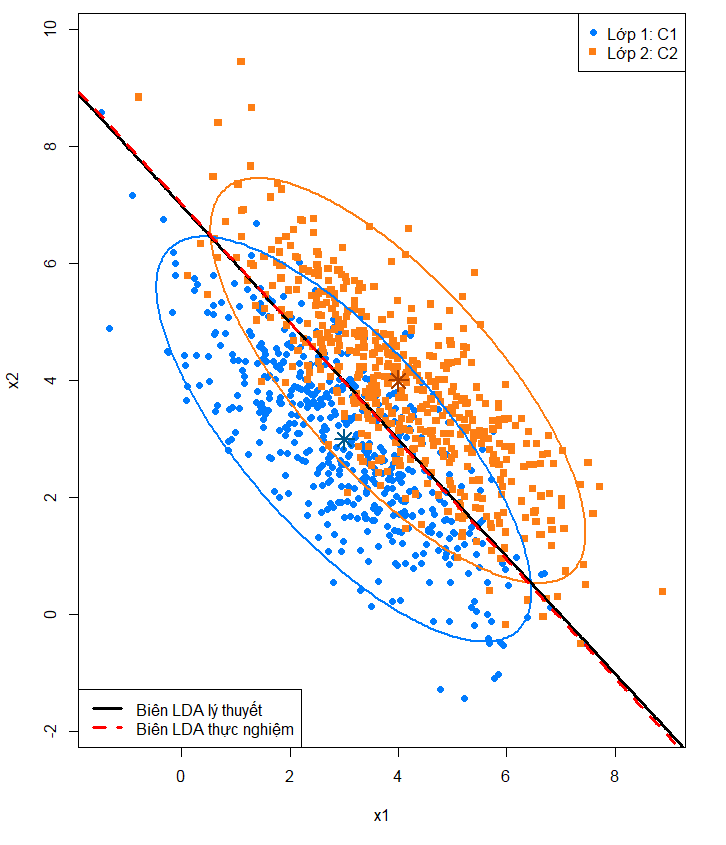
\includegraphics[width=0.8\textwidth]{image/normal_dis_2_classes_test.png}
    \caption{Phân bố mẫu của hai lớp chuẩn hai chiều và biên phân loại LDA.}
    \label{fig:2d_normal_class}
\end{figure}

\clearpage

Để đánh giá kết quả phân loại, ta sử dụng ma trận lỗi.
\begin{figure}[H]
    \centering
    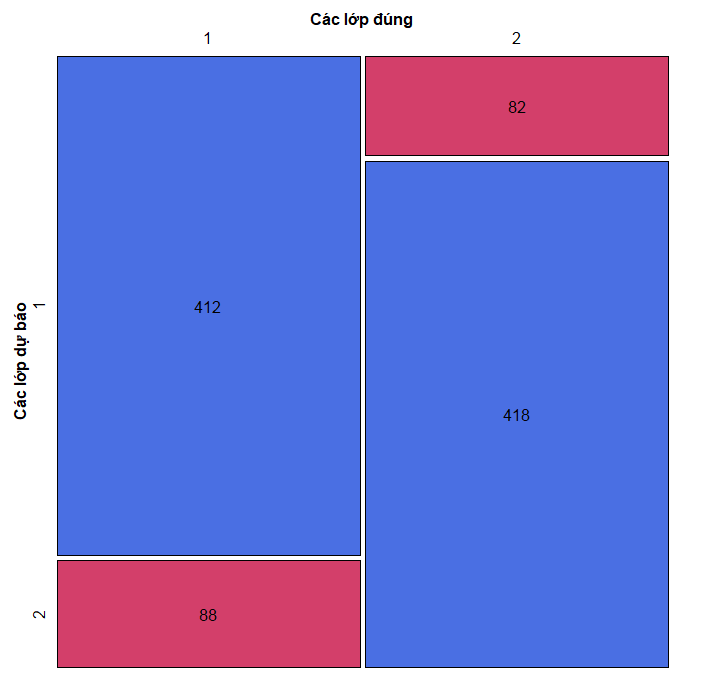
\includegraphics[width=0.6\textwidth]{image/confusion_matrix_test.png}
    \caption{Ma trận lỗi dùng để đánh giá kết quả phân loại của mô hình LDA.}
    \label{fig:confusion_matrix_lda}
\end{figure}

Từ ma trận lỗi hiển thị trên Hình \ref{fig:confusion_matrix_lda}, ta xác định được số lượng các mẫu phân loại đúng và phân loại sai tương ứng của hai lớp. Cụ thể, số mẫu thuộc lớp $C_1$ phân loại đúng là $n_{11} = 412$, số mẫu phân loại sai sang lớp $C_2$ là $n_{21} = 88$. Đối với lớp $C_2$, số mẫu phân loại đúng là $n_{22} = 418$ và số mẫu phân loại sai sang lớp $C_1$ là $n_{12} = 82$.

Tỷ lệ lỗi thực nghiệm (Tỷ lệ phân loại lỗi - $\widehat{\mathrm{TPM}}$) được tính toán cụ thể như sau
\[
\widehat{\mathrm{TPM}}
=
\frac{n_{12}+n_{21}}{n}
=
\frac{82 + 88}{1000}
=
\frac{170}{1000}
=
0{,}170 \quad (17{,}0\%).
\]
Độ chính xác tổng thể của sự phân lớp (the overall accuracy) của mô hình LDA đạt
\[
\text{Overall Accuracy}
=
1 - \widehat{\mathrm{TPM}}
=
1 - 0{,}170
=
0{,}830 \quad (83{,}0\%).
\]
Các chỉ số độ chính xác phân loại (Recall) và độ chính xác tiên đoán (Precision) cho từng lớp $C_j$ ($j = 1, 2$) được xác định theo các công thức
\begin{itemize}
	\item \textbf{Recall:} $P(\hat{C}_j\mid C_j) = \frac{n_{jj}}{n_{\bullet j}}$
	\item \textbf{Precision:} $P(C_j\mid \hat{C}_j) = \frac{n_{jj}}{n_{j\bullet}}$
\end{itemize}

Kết quả tính toán cụ thể được tóm tắt trong Bảng \ref{tab:metrics_summary}

\begin{table}[H]
	\centering
	\renewcommand{\arraystretch}{1.5}
	\begin{tabular}{|c|c|c|}
		\hline
		\textbf{Lớp} & \textbf{Recall} $P(\hat{C}_j \mid C_j)$ & \textbf{Precision} $P(C_j \mid \hat{C}_j)$ \\
		\hline
		\textbf{$C_1$} & $\frac{412}{500} = 82{,}4\%$ & $\frac{412}{494} \approx 83{,}40\%$ \\
		\hline
		\textbf{$C_2$} & $\frac{418}{500} = 83{,}6\%$ & $\frac{418}{506} \approx 82{,}61\%$ \\
		\hline
	\end{tabular}
	\caption{Các chỉ số Recall và Precision cho trường hợp hai lớp ít chồng lấp}
	\label{tab:metrics_summary}
\end{table}

Từ ma trận lỗi theo tần số, ta tính được các tỷ lệ tương ứng bằng công thức
\[
p_{ij}=\frac{n_{ij}}{n},\qquad i,j=1,2.
\]

Với $n=1000$, ta có
\[
p_{11}=\frac{412}{1000}=0{,}412,\qquad
p_{12}=\frac{82}{1000}=0{,}082,
\]
\[
p_{21}=\frac{88}{1000}=0{,}088,\qquad
p_{22}=\frac{418}{1000}=0{,}418.
\]

Ngoài ra,
\[
p_{1\bullet}=p_{11}+p_{12}=0{,}412+0{,}082=0{,}494,
\]
\[
p_{2\bullet}=p_{21}+p_{22}=0{,}088+0{,}418=0{,}506,
\]
và
\[
p_{\bullet 1}=p_{11}+p_{21}=0{,}412+0{,}088=0{,}500,
\]
\[
p_{\bullet 2}=p_{12}+p_{22}=0{,}082+0{,}418=0{,}500.
\]

Do đó, ma trận lỗi theo tỷ lệ được cho bởi bảng sau
\begin{table}[H]
	\centering
	\begin{tabular}{|c|cc|c|}
		\hline
		\multirow{2}{*}{Các lớp dự báo} 
		& \multicolumn{2}{c|}{Các lớp đúng} 
		& \multirow{2}{*}{Tổng cộng} \\ \cline{2-3}
		& $C_1$ & $C_2$ & \\ \hline
		$\hat{C}_1$ & $0{,}412$ & $0{,}082$ & $0{,}494$ \\
		$\hat{C}_2$ & $0{,}088$ & $0{,}418$ & $0{,}506$ \\ \hline
		Tổng cộng & $0{,}500$ & $0{,}500$  & $1{,}000$ \\ \hline
	\end{tabular}
	\caption{Ma trận lỗi theo tỷ lệ của mô hình LDA trong trường hợp hai lớp ít chồng lấp.}
	\label{tab:MaTranLoiTyLe_LDA_ItChongLap}
\end{table}

Trong phần trước, ta đã xét trường hợp hai lớp chuẩn hai chiều có vùng giao nhau nhất định. Để thấy rõ hơn hạn chế của bộ phân loại tuyến tính khi dữ liệu có mức độ chồng lấn cao, ta tiếp tục xét một mô phỏng khác, trong đó hai lớp có tâm rất gần nhau và có cùng ma trận hiệp phương sai.

\subsection{Mô phỏng trường hợp hai lớp chồng lấp nhiều}
Xét bài toán phân loại với dữ liệu hai chiều $(d=2)$. Dữ liệu được sinh ngẫu nhiên từ hai phân phối chuẩn hai chiều có cùng ma trận hiệp phương sai.

Thiết lập các tham số của dữ liệu mô phỏng như sau
\[
n_1=n_2=500.
\]
\[
\bm{\mu}_1=
\begin{pmatrix}
	3\\
	3
\end{pmatrix},
\qquad
\bm{\mu}_2=
\begin{pmatrix}
	3{,}2\\
	2{,}5
\end{pmatrix}.
\]
\[
\Sigma
=
\begin{pmatrix}
	2 & 1\\
	1 & 2
\end{pmatrix}.
\]
Từ các tham số đã thiết lập, ta đã tính được
\[
\bm{\beta}_{\text{opt}}
=
\Sigma^{-1}(\bm{\mu}_1-\bm{\mu}_2)
=
\begin{pmatrix}
	-0{,}3\\
	0{,}4
\end{pmatrix}.
\]

Do hai lớp có xác suất tiên nghiệm bằng nhau, biên LDA lý thuyết đi qua trung điểm của hai vectơ trung bình
\[
\frac{\bm{\mu}_1+\bm{\mu}_2}{2}
=
\begin{pmatrix}
	3{,}1\\
	2{,}75
\end{pmatrix}.
\]

Vì vậy, biên LDA lý thuyết được xác định bởi
\[
\bm{\beta}_{\text{opt}}^T
\left(
\bm{x}_{\text{bnd}}
-
\frac{\bm{\mu}_1+\bm{\mu}_2}{2}
\right)
=
0.
\]

Thay các giá trị đã tính vào, ta có
\[
\begin{pmatrix}
	-0{,}3 & 0{,}4
\end{pmatrix}
\left[
\begin{pmatrix}
	x_1\\
	x_2
\end{pmatrix}
-
\begin{pmatrix}
	3{,}1\\
	2{,}75
\end{pmatrix}
\right]
=
0.
\]

Suy ra phương trình biên LDA lý thuyết là
\[
-0{,}3x_1+0{,}4x_2-0{,}17=0.
\]

Tương đương,
\[
x_2=0{,}425+0{,}75x_1.
\]

Biên LDA lý thuyết này được dùng để so sánh với biên LDA thực nghiệm được ước lượng từ dữ liệu mô phỏng.

Từ các tham số mô phỏng trên, ta sinh ngẫu nhiên tập dữ liệu của hai lớp
\[
D_1=\{\bm{x}_{11},\bm{x}_{21},\ldots,\bm{x}_{n_1 1}\},
\qquad
D_2=\{\bm{x}_{12},\bm{x}_{22},\ldots,\bm{x}_{n_2 2}\}.
\]

Từ dữ liệu mô phỏng, ta tính trung bình mẫu \(\hat{\bm{\mu}}_1, \hat{\bm{\mu}}_2\) và ma trận hiệp phương sai mẫu của từng lớp. \[ \hat{\pi}_1=\hat{\pi}_2=0{,}5, \] \[ \hat{\bm{\mu}}_1 = \begin{pmatrix} 2{,}9716\\ 3{,}0225 \end{pmatrix}, \qquad \hat{\bm{\mu}}_2 = \begin{pmatrix} 3{,}2101\\ 2{,}5101 \end{pmatrix}, \] 
Ma trận hiệp phương sai mẫu của lớp 1 và lớp 2 lần lượt là \[ \hat{\Sigma}_1 = \begin{pmatrix} 2{,}1251 & 0{,}9023\\ 0{,}9023 & 1{,}9656 \end{pmatrix}, \qquad \hat{\Sigma}_2 = \begin{pmatrix} 1{,}7762 & 0{,}8397\\ 0{,}8397 & 1{,}9534 \end{pmatrix}. \] Từ đó, ma trận hiệp phương sai mẫu gộp được ước lượng bởi \[ \hat{\Sigma} = \begin{pmatrix} 1{,}9507 & 0{,}8710\\ 0{,}8710 & 1{,}9595 \end{pmatrix}. \]
Khi đó, phương chiếu Fisher thực nghiệm được xác định bởi \[ \bm{b}_{\text{opt}} = \hat{\Sigma}^{-1}(\hat{\bm{\mu}}_1-\hat{\bm{\mu}}_2) = \begin{pmatrix} -0{,}2982\\ 0{,}3940 \end{pmatrix}. \] Đường phân loại tuyến tính của LDA có dạng \[ \bm{b}_{\text{opt}}^T \left( \bm{x}_{\text{bnd}} - \frac{\hat{\bm{\mu}}_1 + \hat{\bm{\mu}}_2}{2} \right) = 0. \] Trung điểm của hai vectơ trung bình mẫu là \[ \frac{\hat{\bm{\mu}}_1+\hat{\bm{\mu}}_2}{2} = \begin{pmatrix} 3{,}0908\\ 2{,}7663 \end{pmatrix}. \] Thay số vào, ta được \[ \begin{pmatrix} -0{,}2982 & 0{,}3940 \end{pmatrix} \left[ \bm{x} - \begin{pmatrix} 3{,}0908\\ 2{,}7663 \end{pmatrix} \right] = 0. \] Tương đương, \[ -0{,}2982x_1+0{,}3940x_2-0{,}1684=0. \] Hay \[ x_2=0{,}4274+0{,}7567x_1. \]

\begin{figure}[H]
	\centering
	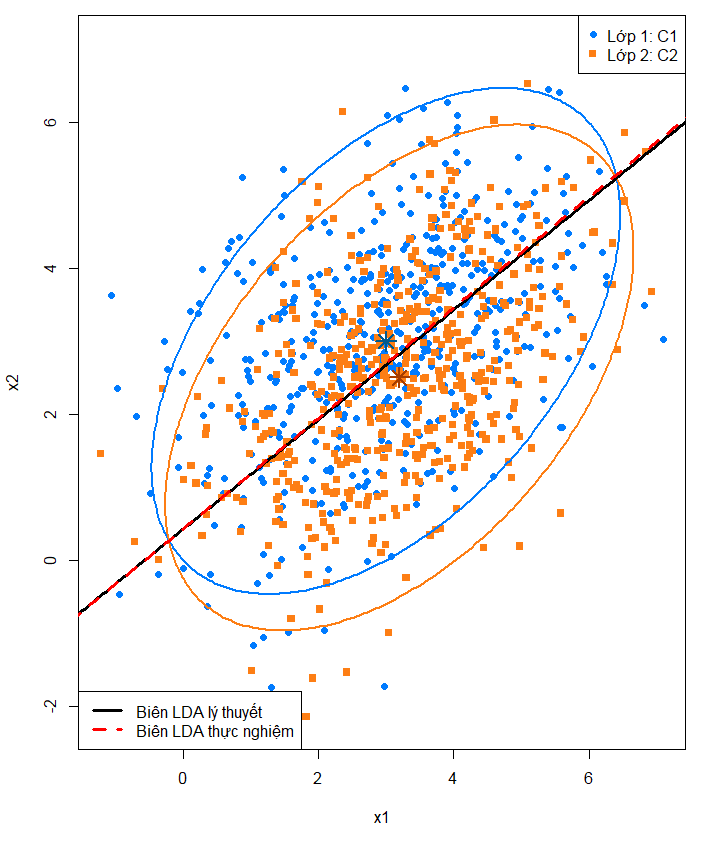
\includegraphics[width=0.8\textwidth]{image/normal_dis_2_classes_overlap_test.png}
	\caption{Phân bố mẫu của hai lớp chuẩn hai chiều có tương quan dương và mức độ chồng lấp lớn.}
	\label{fig:2d_normal_overlap}
\end{figure}

Từ Hình~\ref{fig:2d_normal_overlap}, có thể thấy hai lớp dữ liệu chồng lấn mạnh trong không gian hai chiều. Nguyên nhân chính là do khoảng cách giữa hai vectơ trung bình \[ \hat{\bm{\mu}}_1 = \begin{pmatrix} 2{,}9716\\ 3{,}0225 \end{pmatrix}, \qquad \hat{\bm{\mu}}_2 = \begin{pmatrix} 3{,}2101\\ 2{,}5101 \end{pmatrix} \] khá nhỏ so với độ phân tán của dữ liệu được xác định bởi ma trận hiệp phương sai mẫu gộp \[ \hat{\Sigma} = \begin{pmatrix} 1{,}9507 & 0{,}8710\\ 0{,}8710 & 1{,}9595 \end{pmatrix}. \] Khoảng cách Euclid giữa hai tâm chỉ là \[ \|\hat{\bm{\mu}}_1-\hat{\bm{\mu}}_2\| = \sqrt{(2{,}9716-3{,}2101)^2+(3{,}0225-2{,}5101)^2} \] \[ = \sqrt{(-0{,}2385)^2+(0{,}5124)^2} = \sqrt{0{,}0569+0{,}2626} = \sqrt{0{,}3195} \approx 0{,}5652. \] Trong khi đó, phương sai theo từng trục đều xấp xỉ \(2\), cho thấy độ phân tán của mỗi lớp tương đối lớn. Vì vậy, mặc dù hai lớp có hai tâm khác nhau, phần lớn các điểm dữ liệu vẫn nằm xen kẽ trong cùng một vùng không gian.

\hspace*{0.5cm}Đường LDA vẫn chia không gian thành hai miền quyết định tuyến tính. Tuy nhiên, do vùng giao nhau giữa hai phân phối quá lớn, nhiều điểm của lớp $C_1$ nằm về phía miền quyết định của lớp $C_2$ và ngược lại. Đây là nguyên nhân làm tăng tỷ lệ phân loại sai.

Để đánh giá kết quả phân loại, ta tiếp tục sử dụng ma trận lỗi.

\begin{figure}[H]
	\centering
	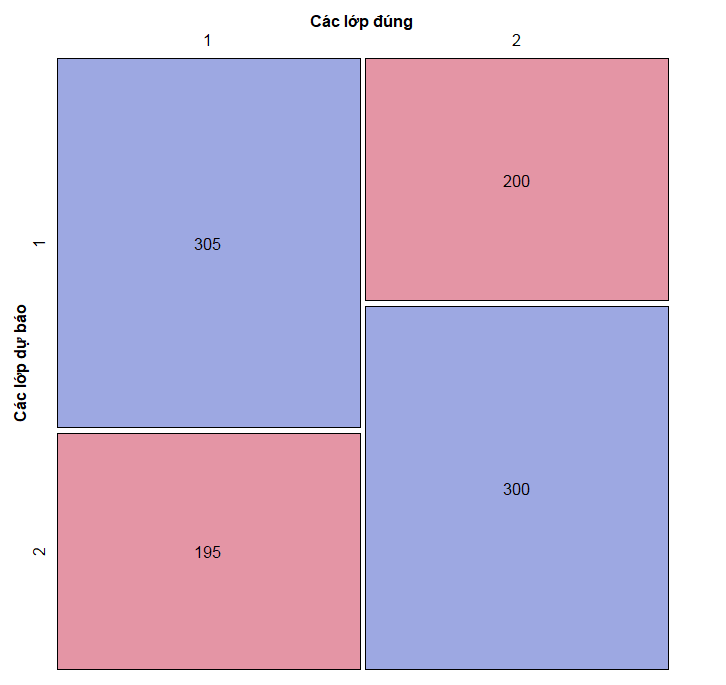
\includegraphics[width=0.6\textwidth]{image/confusion_matrix_overlap_test.png}
	\caption{Ma trận lỗi của mô hình LDA trong trường hợp hai lớp chồng lấp nhiều.}
	\label{fig:confusion_matrix_overlap}
\end{figure}

Từ ma trận lỗi hiển thị trên Hình~\ref{fig:confusion_matrix_overlap}, ta xác định được số lượng các mẫu phân loại đúng và phân loại sai tương ứng của hai lớp. Cụ thể, số mẫu thuộc lớp $C_1$ phân loại đúng là $n_{11}=305$, số mẫu phân loại sai sang lớp $C_2$ là $n_{21}=195$. Đối với lớp $C_2$, số mẫu phân loại đúng là $n_{22}=300$ và số mẫu phân loại sai sang lớp $C_1$ là $n_{12}=200$.

Tỷ lệ lỗi thực nghiệm được tính bởi
\[
\widehat{\mathrm{TPM}}
=
\frac{n_{12}+n_{21}}{n}
=
\frac{200+195}{1000}
=
\frac{395}{1000}
=
0{,}395.
\]

Hay tương đương,
\[
\widehat{\mathrm{TPM}}=39{,}5\%.
\]

Độ chính xác phân loại toàn cục của mô hình LDA là
\[
\text{Overall Accuracy}
=
1-\widehat{\mathrm{TPM}}
=
1-0{,}395
=
0{,}605.
\]

Hay,
\[
\text{Overall Accuracy}=60{,}5\%.
\]
Các chỉ số độ chính xác phân loại (Recall) và độ chính xác tiên đoán (Precision) cho từng lớp $C_j$ ($j = 1, 2$) được xác định theo các công thức:
\begin{itemize}
	\item \textbf{Recall:} $P(\hat{C}_j\mid C_j) = \frac{n_{jj}}{n_{\bullet j}}$
	\item \textbf{Precision:} $P(C_j\mid \hat{C}_j) = \frac{n_{jj}}{n_{j\bullet}}$
\end{itemize}

Kết quả tính toán cụ thể được tóm tắt trong Bảng \ref{tab:metrics_summary}

\begin{table}[htpb]
	\centering
	\renewcommand{\arraystretch}{1.5}
	\begin{tabular}{|c|c|c|}
		\hline
		\textbf{Lớp} & \textbf{Recall} $P(\hat{C}_j \mid C_j)$ & \textbf{Precision} $P(C_j \mid \hat{C}_j)$ \\
		\hline
		\textbf{$C_1$} & $\frac{305}{500} = 61{,}0\%$ & $\frac{305}{505} \approx 60{,}40\%$ \\
		\hline
		\textbf{$C_2$} & $\frac{300}{500} = 60{,}0\%$ & $\frac{300}{495} \approx 60{,}61\%$ \\
		\hline
	\end{tabular}
	\caption{Các chỉ số Recall và Precision cho trường hợp hai lớp chồng lấp nhiều}
	\label{tab:metrics_summary}
\end{table}

Từ ma trận lỗi theo tần số, ta tính được các tỷ lệ tương ứng bằng công thức $p_{ij} = \frac{n_{ij}}{n}$ ($i,j=1,2$). Với $n=1000$, ta có các tỷ lệ thành phần và các tổng lề như sau
\begin{align*}
	p_{11} &= \frac{305}{1000} = 0{,}305, & p_{12} &= \frac{200}{1000} = 0{,}200, & p_{1\bullet} &= 0{,}305 + 0{,}200 = 0{,}505 \\
	p_{21} &= \frac{195}{1000} = 0{,}195, & p_{22} &= \frac{300}{1000} = 0{,}300, & p_{2\bullet} &= 0{,}195 + 0{,}300 = 0{,}495 \\
	p_{\bullet 1} &= 0{,}305 + 0{,}195 = 0{,}500, & p_{\bullet 2} &= 0{,}200 + 0{,}300 = 0{,}500
\end{align*}

Do đó, ma trận lỗi theo tỷ lệ được cho bởi bảng sau
\begin{table}[H]
	\centering
	\begin{tabular}{|c|cc|c|}
		\hline
		\multirow{2}{*}{Các lớp dự báo} 
		& \multicolumn{2}{c|}{Các lớp đúng} 
		& \multirow{2}{*}{Tổng cộng} \\ \cline{2-3}
		& $C_1$ & $C_2$ & \\ \hline
		$\hat{C}_1$ & $0{,}305$ & $0{,}200$ & $0{,}505$ \\
		$\hat{C}_2$ & $0{,}195$ & $0{,}300$ & $0{,}495$ \\ \hline
		Tổng cộng & $0{,}500$ & $0{,}500$  & $1{,}000$ \\ \hline
	\end{tabular}
	\caption{Ma trận lỗi theo tỷ lệ của mô hình LDA trong trường hợp hai lớp chồng lấp nhiều.}
	\label{tab:MaTranLoiTyLe_LDA_ChongLanNhieu}
\end{table}

Kết quả này cho thấy khi hai lớp có mức độ chồng lấn lớn, hiệu quả phân loại của LDA giảm đáng kể. Mặc dù LDA vẫn xác định được một đường phân loại tuyến tính, đường này không thể tách hoàn toàn hai lớp do phần lớn các quan sát của hai lớp nằm xen kẽ trong cùng một vùng không gian. Sai số phân loại $39{,}5\%$ phản ánh mức độ khó của bài toán, xuất phát từ việc hai phân phối có tâm rất gần nhau so với độ phân tán của dữ liệu. Trong trường hợp này, sai số không chủ yếu đến từ việc lựa chọn sai dạng mô hình, vì hai lớp vẫn được sinh từ các phân phối chuẩn có cùng ma trận hiệp phương sai. Nguyên nhân chính là vùng chồng lấn giữa hai phân phối quá lớn, làm cho nhiều điểm thuộc lớp $C_1$ có đặc trưng gần giống với lớp $C_2$ và ngược lại. Do đó, ngay cả biên quyết định tuyến tính tối ưu theo LDA cũng không thể đạt độ chính xác cao.

\hspace*{0.5cm}Trường hợp mô phỏng này cho thấy khi hai phân phối chuẩn có tâm quá gần nhau so với độ phân tán nội tại, vùng chồng lấn giữa hai lớp trở nên rất lớn. Khi đó, ngay cả khi giả thiết của LDA được thỏa mãn, tức là hai lớp có cùng ma trận hiệp phương sai và biên Bayes là tuyến tính, mô hình vẫn không thể phân loại tốt.

Qua các mô phỏng trên, có thể thấy hiệu quả của phương pháp Fisher LDA phụ thuộc mạnh vào cấu trúc phân bố của dữ liệu. Khi hai lớp có tâm cách xa nhau và mức độ chồng lấn nhỏ, LDA xác định được một biên phân loại tuyến tính tương đối tốt, cho tỷ lệ phân loại sai thấp. Ngược lại, khi hai lớp có tâm gần nhau, phương sai lớn hoặc vùng chồng lấn giữa hai phân phối trở nên đáng kể, tỷ lệ lỗi phân loại tăng lên rõ rệt.

\hspace*{0.5cm}Trường hợp hai lớp chồng lấn ít trong ví dụ đầu cho thấy LDA có thể đạt độ chính xác khá cao, chẳng hạn tỷ lệ lỗi thực nghiệm khoảng $17{,}0\%$. Trong khi đó, ở trường hợp hai lớp chồng lấn mạnh, tỷ lệ lỗi tăng lên đến $39{,}5\%$, tương ứng độ chính xác chỉ còn $60{,}5\%$. Sự khác biệt này minh họa rõ rằng khả năng phân tách của LDA không chỉ phụ thuộc vào việc có tồn tại biên tuyến tính hay không, mà còn phụ thuộc vào mức độ tách biệt thực sự giữa các phân phối lớp.

\hspace*{0.5cm}Như vậy, Fisher LDA là một phương pháp hiệu quả khi dữ liệu có cấu trúc lớp tương đối rõ ràng và thỏa mãn các giả thiết của mô hình. Tuy nhiên, trong các bài toán mà các lớp chồng lấn mạnh, ngay cả biên tuyến tính tối ưu cũng khó đạt hiệu quả phân loại cao. Điều này cho thấy khi áp dụng LDA trong thực hành, cần xem xét đồng thời các yếu tố như khoảng cách giữa các tâm lớp, độ phân tán của dữ liệu các nhóm.


\subsection{Mô phỏng trường hợp hai lớp tách biệt hoàn toàn}

Xét bài toán phân loại với dữ liệu hai chiều $(d=2)$ tương tự nhưng trong điều kiện hai phân phối có khoảng cách tâm (trung bình) đủ lớn.

Thiết lập các tham số của dữ liệu mô phỏng như sau
\[
n_1=n_2=500.
\]
\[
\bm{\mu}_1=
\begin{pmatrix}
	3\\
	3
\end{pmatrix},
\qquad
\bm{\mu}_2=
\begin{pmatrix}
	13\\
	3
\end{pmatrix}.
\]
\[
\Sigma
=
\begin{pmatrix}
	2 & 0\\
	0 & 2
\end{pmatrix}.
\]

Do các phần tử ngoài đường chéo của ma trận hiệp phương sai bằng $0$, ta có
\[
\sigma_{12}=\sigma_{21}=0.
\]
Điều này cho thấy hai biến đặc trưng $x_1$ và $x_2$ không có tương quan tuyến tính. Đồng thời, do hai phần tử trên đường chéo chính bằng nhau, tức là
\[
\sigma_1^2=\sigma_2^2=2,
\]
nên mức độ phân tán theo hai hướng $x_1$ và $x_2$ là như nhau. Vì vậy, các đám mây điểm của hai lớp có dạng gần tròn.

Trong trường hợp này, do hai lớp có cùng ma trận hiệp phương sai và cùng xác suất tiên nghiệm, biên quyết định LDA tương ứng với tập hợp các điểm có khoảng cách Mahalanobis đến hai tâm bằng nhau. Tuy nhiên, vì
\[
\Sigma=2\mathbb{I},
\]
khoảng cách Mahalanobis chỉ khác khoảng cách Euclid một hệ số tỷ lệ. Do đó, biên quyết định LDA chính là đường trung trực của đoạn nối hai tâm $\bm{\mu}_1$ và $\bm{\mu}_2$.


Trung điểm của hai vectơ trung bình là
\[
\bm{M}
=
\frac{\bm{\mu}_1+\bm{\mu}_2}{2}
=
\begin{pmatrix}
	\frac{3+13}{2}\\
	\frac{3+3}{2}
\end{pmatrix}
=
\begin{pmatrix}
	8\\
	3
\end{pmatrix}.
\]

Vì hai tâm có cùng tung độ và chỉ khác nhau theo phương $x_1$, đoạn nối hai tâm là một đoạn thẳng nằm ngang. Do đó, đường trung trực của đoạn nối hai tâm là đường thẳng đứng đi qua hoành độ của trung điểm:
\[
x_1=8.
\]

Mặt khác, từ dữ liệu mô phỏng, ta tính trung bình mẫu \(\hat{\bm{\mu}}_1, \hat{\bm{\mu}}_2\). 
\[
\hat{\pi}_1=\hat{\pi}_2=0{,}5.
\]
\[
\hat{\bm{\mu}}_1
=
\begin{pmatrix}
	2{,}9491\\
	2{,}9966
\end{pmatrix},
\qquad
\hat{\bm{\mu}}_2
=
\begin{pmatrix}
	12{,}9999\\
	3{,}0117
\end{pmatrix}.
\]
Ma trận hiệp phương sai mẫu ước lượng của lớp $1$ và lớp $2$ lần lượt là \[ \hat{\Sigma}_1 = \begin{pmatrix} 2{,}2861 & 0{,}0921\\ 0{,}0921 & 1{,}9651 \end{pmatrix}, \qquad \hat{\Sigma}_2 = \begin{pmatrix} 2{,}0503 & -0{,}1023\\ -0{,}1023 & 1{,}8030 \end{pmatrix}. \] Từ hai ma trận hiệp phương sai mẫu trên, ta thu được ma trận hiệp phương sai mẫu gộp \[ \hat{\Sigma} = \begin{pmatrix} 2{,}1682 & -0{,}0051\\ -0{,}0051 & 1{,}8841 \end{pmatrix}. \]

Khi đó, phương chiếu Fisher thực nghiệm được xác định bởi
\[
\bm{b}_{\text{opt}}
=
\hat{\Sigma}^{-1}
(\hat{\bm{\mu}}_1-\hat{\bm{\mu}}_2)
=
\begin{pmatrix}
	-4{,}6356\\
	-0{,}0205
\end{pmatrix}.
\]

Đường phân loại tuyến tính của LDA có dạng
\[
\bm{b}_{\text{opt}}^T
\left(
\bm{x}_{\text{bnd}}
-
\frac{\hat{\bm{\mu}}_1+\hat{\bm{\mu}}_2}{2}
\right)
=0.
\]

Trung điểm của hai vectơ trung bình mẫu là
\[
\frac{\hat{\bm{\mu}}_1+\hat{\bm{\mu}}_2}{2}
=
\begin{pmatrix}
	7{,}9745\\
	3{,}0041
\end{pmatrix}.
\]

Thay số vào, ta được
\[
\begin{pmatrix}
	-4{,}6356 & -0{,}0205
\end{pmatrix}
\left[
\bm{x}
-
\begin{pmatrix}
	7{,}9745\\
	3{,}0041
\end{pmatrix}
\right]
=0.
\]

Tương đương, phương trình biên LDA thực nghiệm là \[ -4{,}6356x_1 - 0{,}0205x_2 + 37{,}0283 = 0. \] Nếu viết dưới dạng \(x_2=a+bx_1\), ta thu được \[ x_2 \approx 1802{,}3010 - 225{,}6309x_1. \] Tuy nhiên, dạng biểu diễn này không thật sự thuận tiện để diễn giải vì hệ số của \(x_2\) trong phương trình tổng quát rất nhỏ so với hệ số của \(x_1\), cụ thể \[ |-0{,}0205| \ll |-4{,}6356|. \] Điều này cho thấy đường biên phân loại gần như là một đường thẳng đứng. Do đó, để thấy rõ vị trí của biên quyết định, ta có thể xấp xỉ bằng cách bỏ qua hạng tử chứa \(x_2\). Khi đó, \[ -4{,}6356x_1+37{,}0283 \approx 0, \] suy ra \[ x_1 \approx \frac{37{,}0283}{4{,}6356} \approx 7{,}9878. \] Như vậy, biên LDA thực nghiệm gần như là đường thẳng đứng đi qua \(x_1 \approx 7{,}9878\), phù hợp với việc hai lớp chủ yếu tách biệt theo trục \(x_1\).

Mặt khác, do ma trận hiệp phương sai mẫu gộp
\[
\hat{\Sigma}
=
\begin{pmatrix}
	2{,}1682 & -0{,}0051\\
	-0{,}0051 & 1{,}8841
\end{pmatrix}
\]
xấp xỉ ma trận $2\mathbb{I}$, nên
\[
\hat{\Sigma}^{-1}
\approx
\frac{1}{2}\mathbb{I}.
\]

Vì vậy,
\[
\bm{b}_{\text{opt}}
=
\hat{\Sigma}^{-1}
(\hat{\bm{\mu}}_1-\hat{\bm{\mu}}_2)
\approx
\frac{1}{2}
(\hat{\bm{\mu}}_1-\hat{\bm{\mu}}_2).
\]
Có
\[
\hat{\bm{\mu}}_1-\hat{\bm{\mu}}_2
=
\begin{pmatrix}
	2{,}9491\\
	2{,}9966
\end{pmatrix}
-
\begin{pmatrix}
	12{,}9999\\
	3{,}0117
\end{pmatrix}
=
\begin{pmatrix}
	-10{,}0508\\
	-0{,}0150
\end{pmatrix},
\]
nên
\[
\bm{b}_{\text{opt}}
\approx
\frac{1}{2}
\begin{pmatrix}
	-10{,}0508\\
	-0{,}0150
\end{pmatrix}
=
\begin{pmatrix}
	-5{,}0254\\
	-0{,}0075
\end{pmatrix}.
\]

Do đó, phương pháp tuyến của biên phân loại cùng phương với đoạn nối hai tâm. Vì đoạn nối hai tâm song song với trục $x_1$, nên biên phân loại vuông góc với trục này và có dạng một đường thẳng đứng.

\begin{figure}[H]
	\centering
	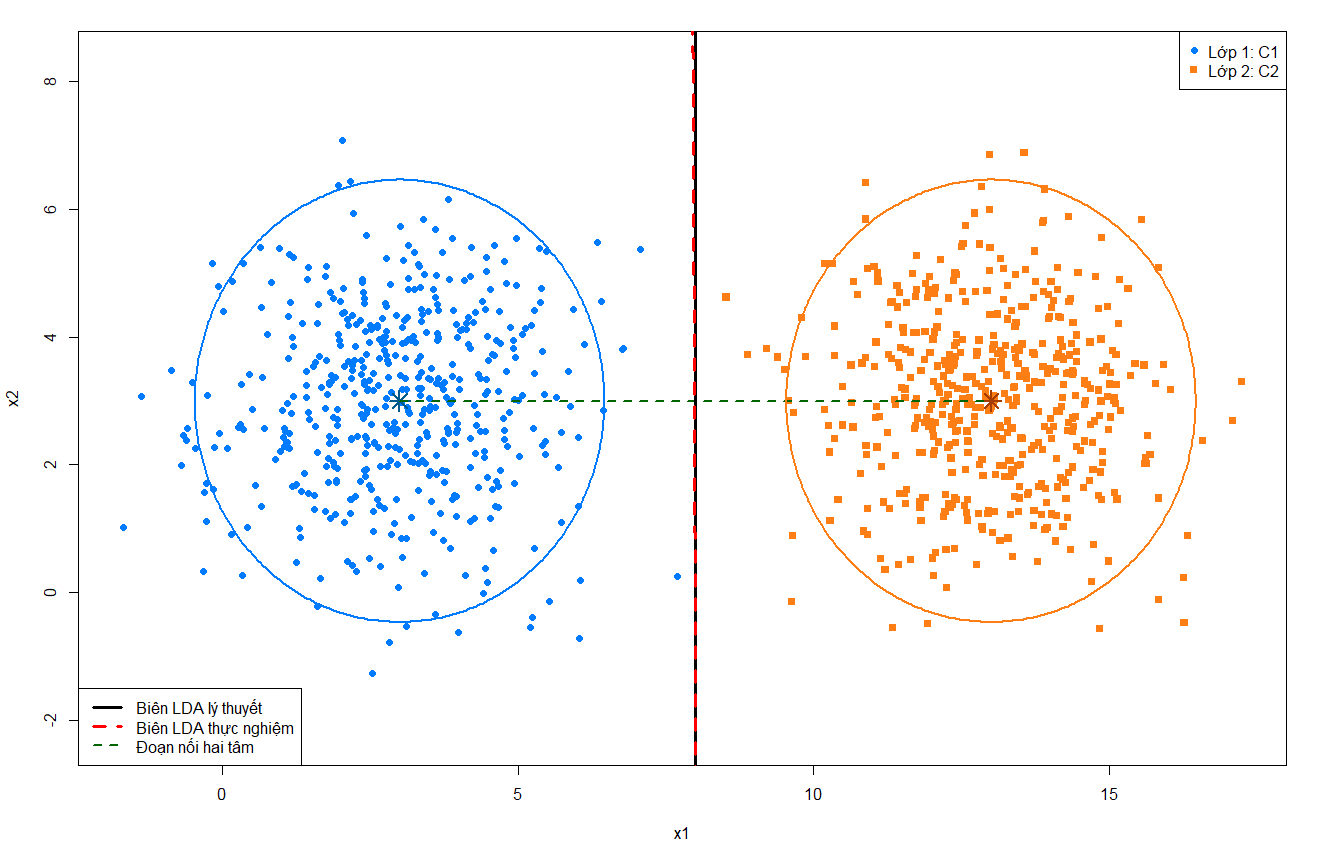
\includegraphics[width=0.75\textwidth]{image/circular_separable_2_classes.png}
	\caption{Hai đám mây chuẩn hai chiều không tương quan, có dạng tròn và được phân tách bởi biên LDA gần với đường trung trực của hai tâm.}
	\label{fig:circular_separable_class}
\end{figure}

Từ Hình~\ref{fig:circular_separable_class}, có thể thấy hai lớp tạo thành hai cụm dữ liệu gần tròn, tách biệt rõ ràng trong không gian hai chiều. Đường phân loại LDA gần như là một đường thẳng đứng nằm giữa hai cụm dữ liệu và gần với đường trung trực của đoạn nối hai tâm. Trong trường hợp này, biên phân loại không chỉ là một đường thẳng tối ưu theo LDA mà còn có ý nghĩa hình học rất trực quan: mỗi điểm dữ liệu được gán vào lớp có tâm gần nó hơn.

Kết quả phân loại cho thấy không có điểm dữ liệu nào bị phân loại sai. Ma trận lỗi thực nghiệm có dạng
\[
\begin{array}{c|cc}
	& \text{Dự đoán } C_1 & \text{Dự đoán } C_2\\
	\hline
	\text{Thực tế } C_1 & 500 & 0\\
	\text{Thực tế } C_2 & 0 & 500
\end{array}
\]
\begin{figure}[H]
	\centering
	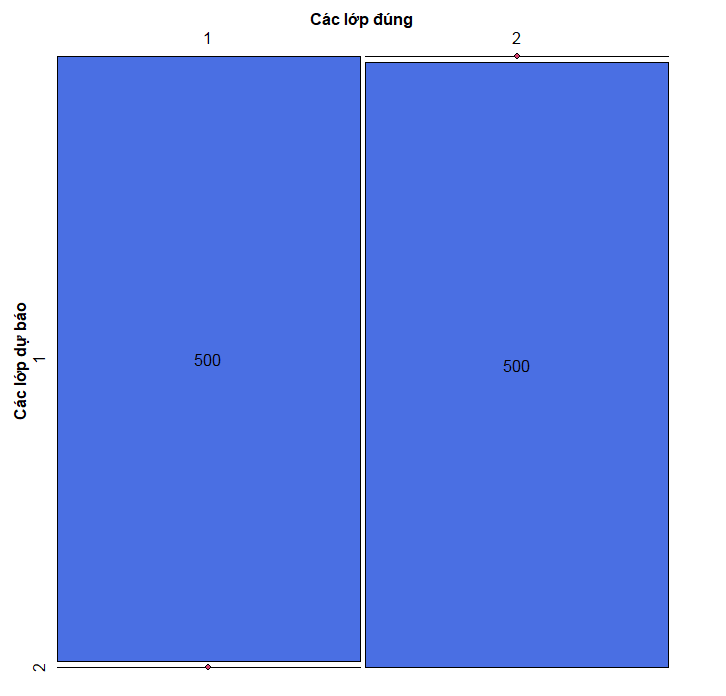
\includegraphics[width=0.75\textwidth]{image/confusion_matrix_separable_test.png}
	\caption{Ma trận lỗi của mô hình LDA trong trường hợp hai lớp tách biệt hoàn toàn.}
	\label{fig:confusion_matrix_separable_test}
\end{figure}
Từ ma trận trên, các phần tử ngoài đường chéo chính đều bằng $0$, tức là
\[
n_{12}=0,\qquad n_{21}=0.
\]

Do đó, tỷ lệ lỗi thực nghiệm là
\[
\widehat{\mathrm{TPM}}
=
\frac{n_{12}+n_{21}}{n}
=
\frac{0+0}{1000}
=
0.
\]

Độ chính xác phân loại đạt
\[
\text{Overall Accuracy}
=
1-\widehat{\mathrm{TPM}}
=
1-0
=
1.
\]

Hay tương đương
\[
\text{Overall Accuracy}=100\%.
\]
Do $n_{12}=n_{21}=0$, không có quan sát nào bị phân loại sai. Vì vậy, đối với cả hai lớp, các chỉ số Recall và Precision đều đạt $100\%$
\[
\text{Recall}_{C_1}
=
\text{Recall}_{C_2}
=
\text{Precision}_{C_1}
=
\text{Precision}_{C_2}
=
100\%.
\]
Kết quả phân loại hoàn hảo này được thể hiện rất rõ qua ma trận lỗi theo tỷ lệ dưới đây
\begin{table}[H]
	\centering
	\begin{tabular}{|c|cc|c|}
		\hline
		\multirow{2}{*}{Các lớp dự báo} 
		& \multicolumn{2}{c|}{Các lớp đúng} 
		& \multirow{2}{*}{Tổng cộng} \\ \cline{2-3}
		& $C_1$ & $C_2$ & \\ \hline
		$\hat{C}_1$ & $0{,}500$ & $0$ & $0{,}500$ \\
		$\hat{C}_2$ & $0$ & $0{,}500$ & $0{,}500$ \\ \hline
		Tổng cộng & $0{,}500$ & $0{,}500$  & $1{,}000$ \\ \hline
	\end{tabular}
	\caption{Ma trận lỗi theo tỷ lệ của mô hình LDA trong trường hợp hai lớp tách biệt hoàn toàn.}
	\label{tab:MaTranLoiTyLe_LDA_TachBietHoanToan}
\end{table}
Trường hợp này cho thấy khi hai lớp có cùng ma trận hiệp phương sai dạng $\sigma^2 \mathbb{I}$, không có tương quan giữa các biến đặc trưng và hai tâm cách xa nhau, LDA đưa ra một biên phân loại rất trực quan: đường trung trực của đoạn nối hai tâm. Đây là một trường hợp đặc biệt trong đó quy tắc phân loại LDA tương đương với quy tắc gán điểm vào lớp có tâm gần nhất theo khoảng cách Euclid. Khi khoảng cách giữa hai tâm đủ lớn so với độ phân tán trong từng lớp, hai đám mây dữ liệu được phân tách hoàn toàn và tỷ lệ lỗi thực nghiệm bằng $0$.